\subsection{Problem}
%%%%%%%%%%%%%%%%%%%%%%%%%%%%%%%%%%%%%%%%%%%%%%%%%%%%%%%%%%%%%%%%%%%%%
\begin{frame}{Motivating Scenarios}
    Fukushima Disaster (2011)
    %\footnote{https://rememberfukushima.org/fallout-maps/}
    \hspace{0.4 cm}
    Deep Water Horizon (2010)
    %\footnote{https://response.restoration.noaa.gov}
    \\
	\begin{minipage}{0.45\textwidth}	
		\begin{figure}
			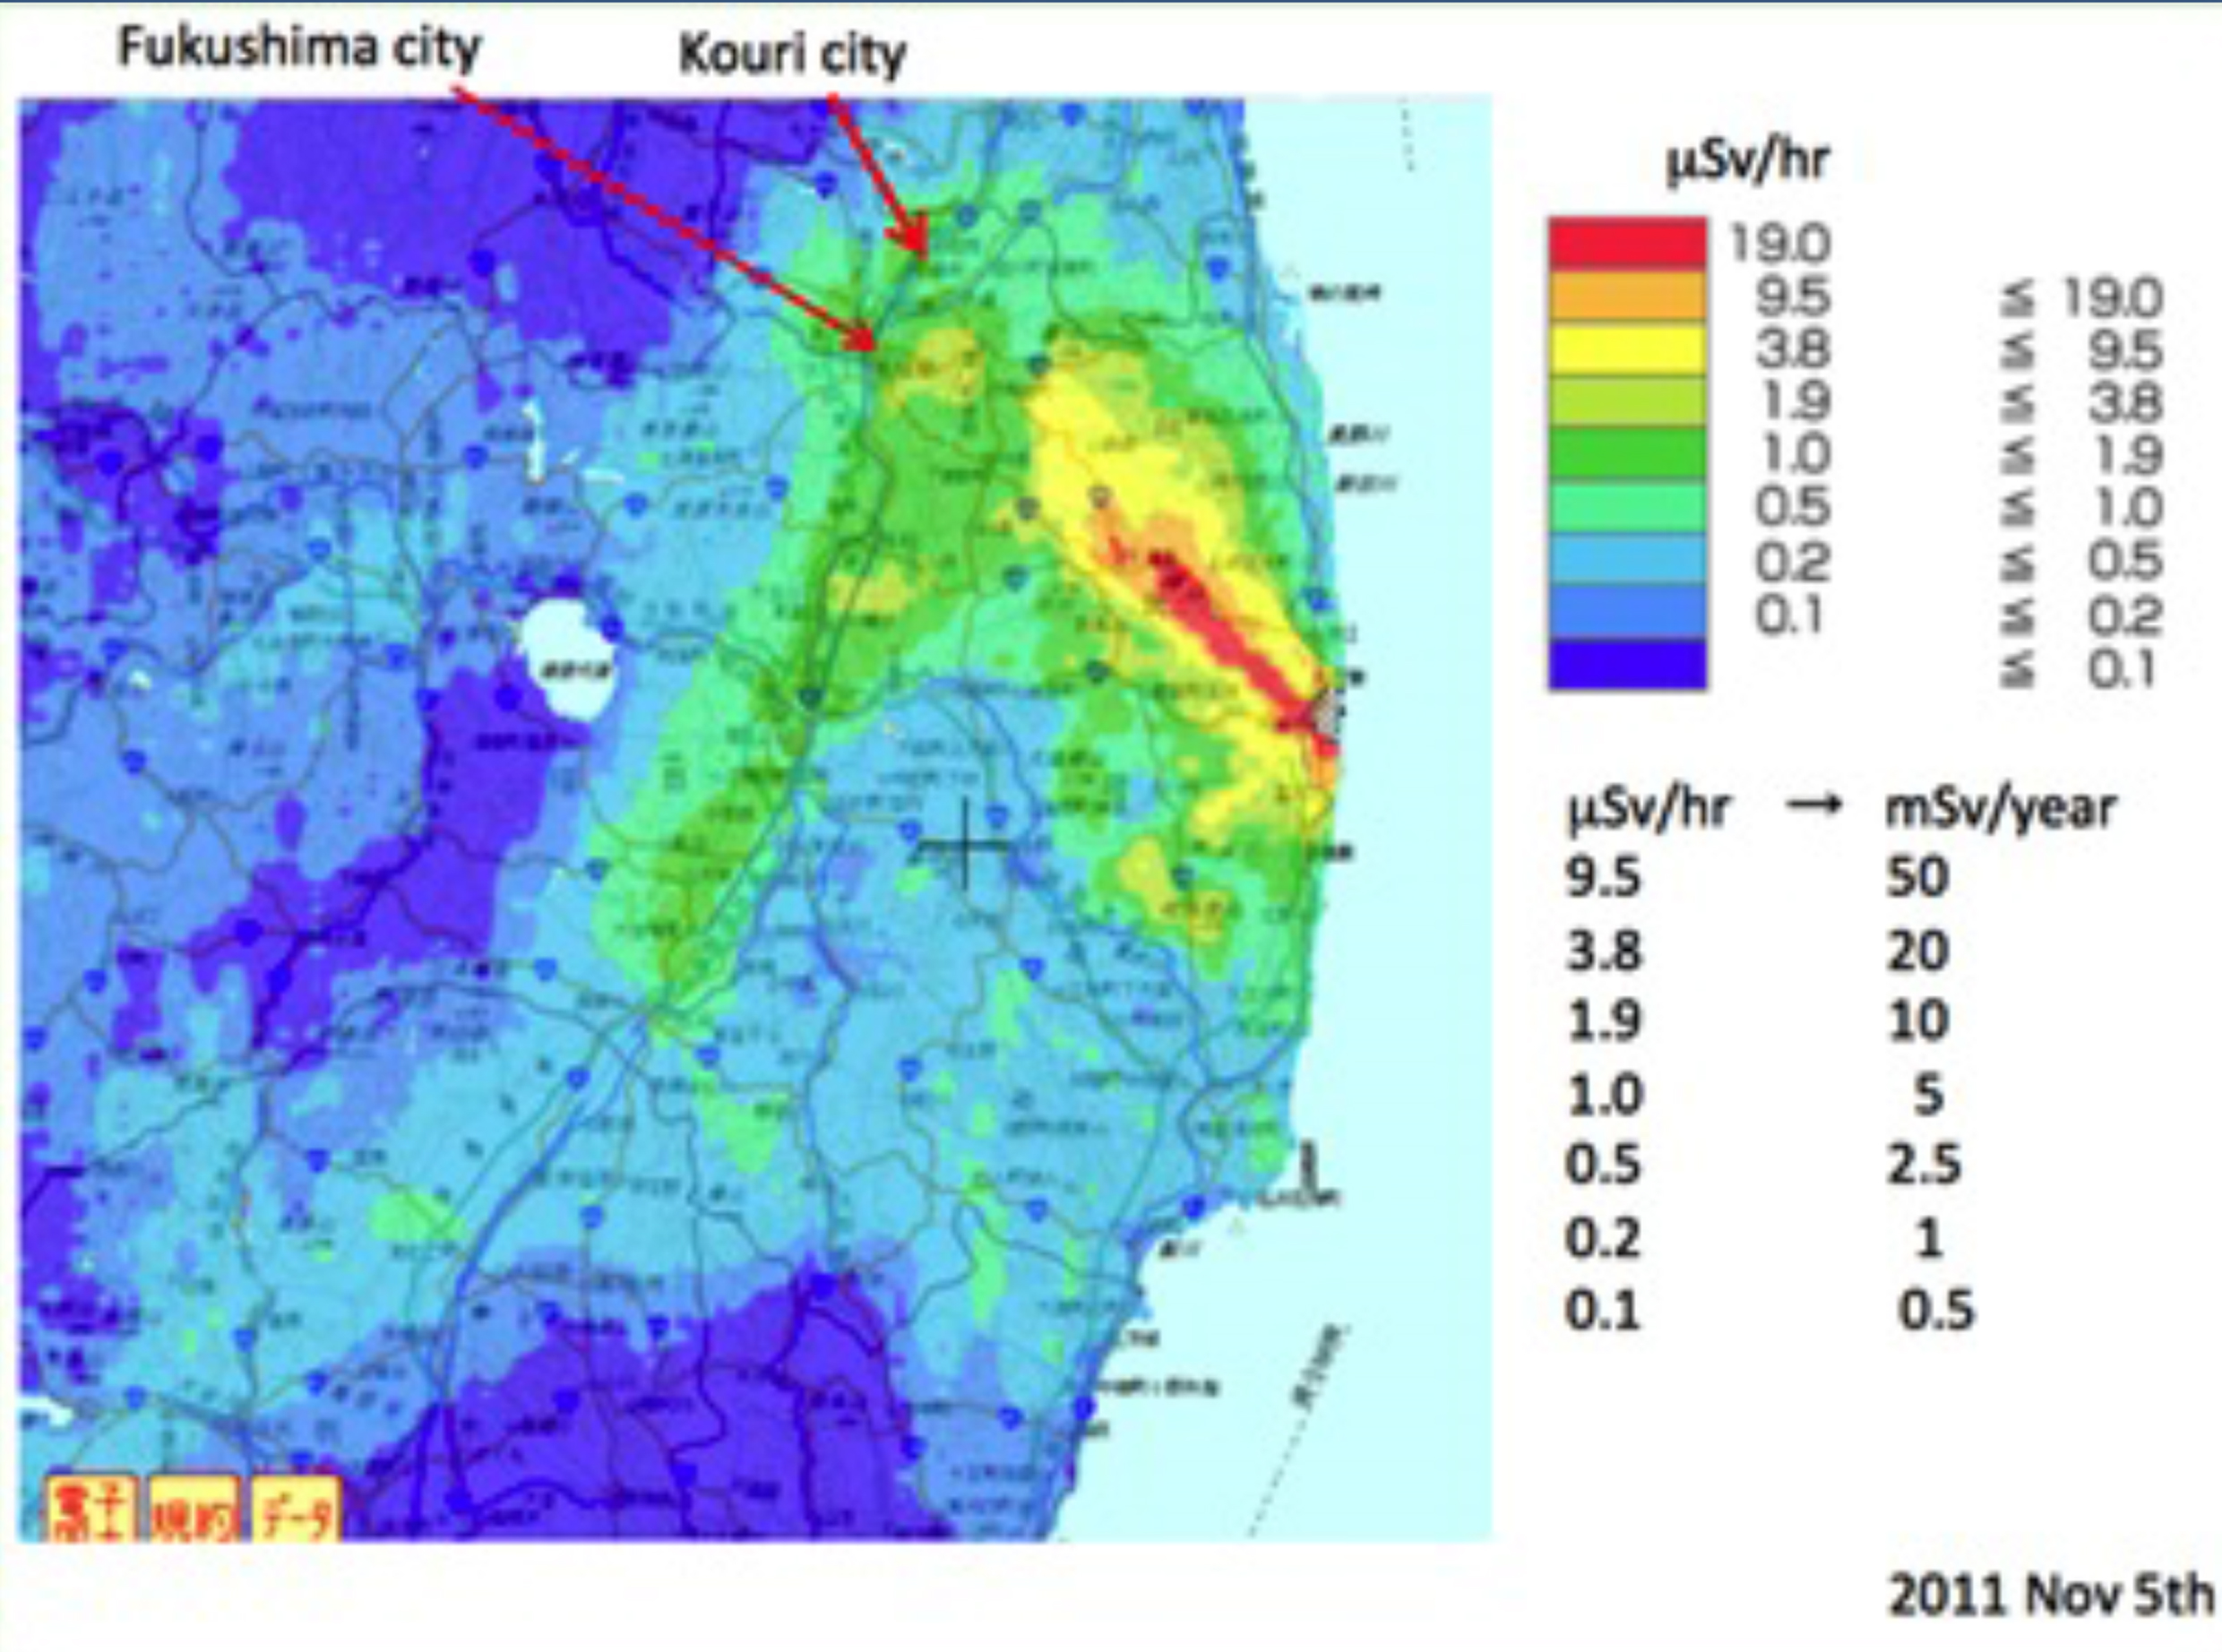
\includegraphics[width=1\textwidth]{figures/fukushima_disaster.jpg}
			%\caption{Fukushima Disaster (2011)}
			%\label{fig:fukushima_disaster}
		\end{figure}
		\begin{figure}
			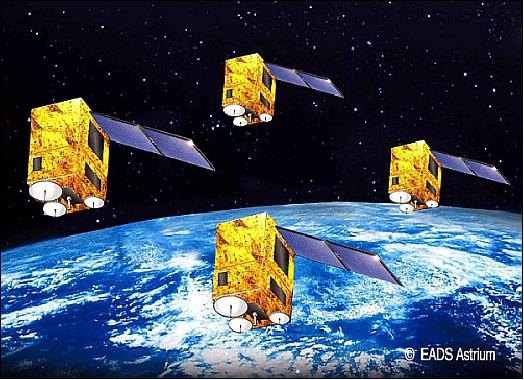
\includegraphics[scale=0.2]{figures/Essaim_constellation.jpg}\label{fig:satellite_flock}
		\end{figure}
	\end{minipage}
	\hspace{0.05cm}
	\begin{minipage}{0.45\textwidth}
		\begin{figure}
			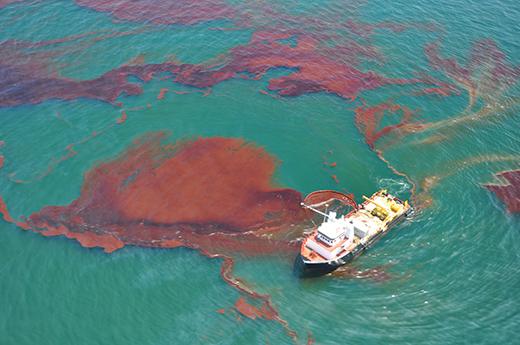
\includegraphics[width=\textwidth]{figures/oil_spill.jpg}
			%\caption{Oil Spills}
			%\label{fig:oilspills}
		\end{figure}
		\begin{figure}
			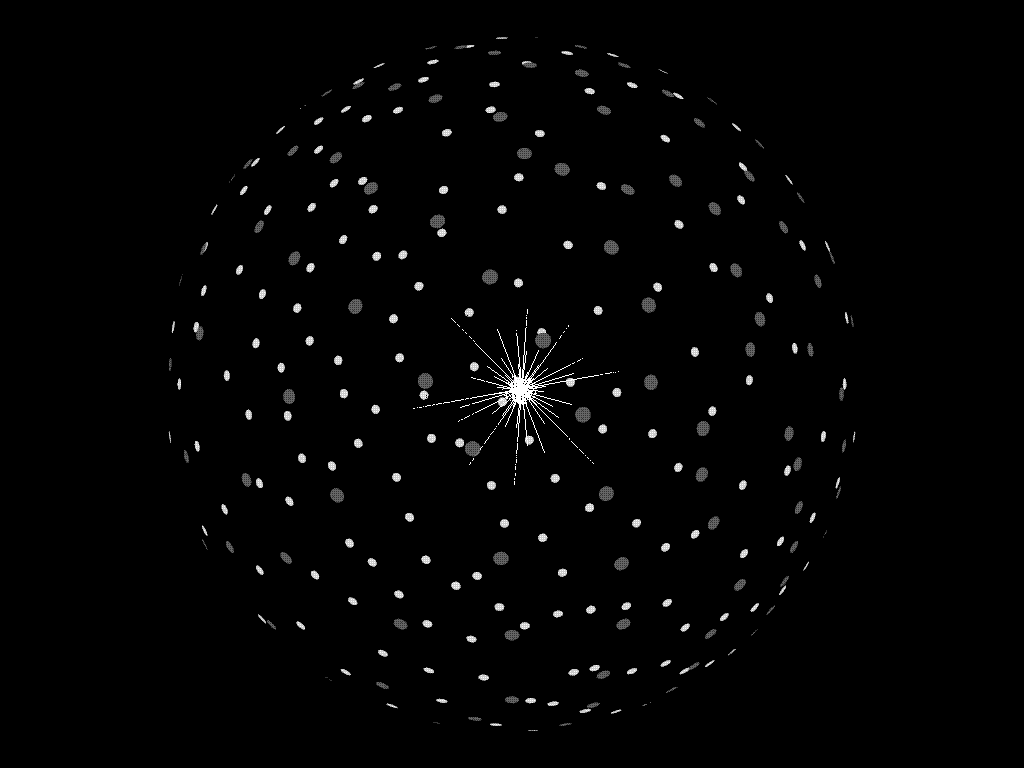
\includegraphics[scale=0.1]{figures/Dyson_swarm.png}		
			\label{fig:Dyson_swarms}
		\end{figure}	
	\end{minipage}
 
 .
 \hspace{0.5 cm}
  EADS Astrium 
 %\footnote{https://earth.esa.int}
\hspace{1.7 cm}
Dyson Swarm (Why not !)
\\
%\vspace{0.5cm}
%\begin{itemize}
%	\item Disaster striken areas could be dangerous and potentially life threatening for humans 
%	\item Deploy a swarm of autonomous robots with sensing and communication capabilities to locate the source of accident.
%\end{itemize}
\end{frame}
%%%%%%%%%%%%%%%%%%%%%%%%%%%%%%%%%%%%%%%%%%%%%%%%%%%%%%%%%%%%%%%%%%%%%
\begin{frame}{Source seeking problem: Abstraction}
	
\begin{itemize}
	\item A group of $N$ agents (e.g underwater robots) are deployed in the region of interest
	\item Each agent has the following properties:
	    \begin{itemize}
	        \item Absolute position measurement (e.g GPS)\footnote{This assumption can be removed as long there is relative displacement measurement}
	        \item Communication with agents within a fixed distance
	        \item Concentration measurement sensor
	        \item Computation capabilities 
	    \end{itemize}
	\item \textbf{Problem:} Design distributed control algorithms that cause the agents to flock towards the source (location with the highest concentration) in a cooperative manner.
\end{itemize}
\end{frame}
%%%%%%%%%%%%%%%%%%%%%%%%%%%%%%%%%%%%%%%%%%%%%%%%%%%%%%%%%%%%%%%%%%%%%
%\begin{frame}{Outline}
%\begin{itemize}
%    \item Drawing motivation from
%    \begin{itemize}
%        \item Momentum methods in Optimization\footnote{Polyak, 1964 and Redont et al., 2002}
%        \item Flocking framework\footnote{Olfati-saber, 2004 and Leonhard, 2003}
%    \end{itemize}
%    Propose a distributed control algorithm to address the source seeking problem.
%    \item Analyze the convergence properties of the proposed algorithm
%    \item Discuss practical aspects and plausibility of assumptions used in analysis
%    \item Present experimental results with small quadrotors in indoor experiments.
%\end{itemize}
%\end{frame}